\chapter{Software Frameworks for Proteomic Data Analysis}

\section{Summary}
Proteomic research can be divided into three major parts: 1) sample generation and preparation, 2) mass spectra collection, and 3) data interpretation and analysis. While improvements in both sample preparation and instrumentation have greatly propelled the field forward, data analysis software has developed at a slower rate. This may be a result of competing standards of data storage and access, the shear complexity of large-scale data, or the simple fact that a majority of scientists are not programmers. Whatever the case may be, automatic data analysis is needed to help answer large and meaningful biological problems. The existence of software is not the final goal; the tools must be simple to use yet powerful, flexible yet robust, accessible yet timely in order to gain traction and be impactful to the field. To meet these demands, the following chapter describes the development of two open-source software packages used in proteomic data analysis. The first package is the Coon OMSSA Proteomic Analysis Software Suite (\compass{}), a graphical interface program used to analyze proteomic data from initial spectral processing all the way to protein quantitation. It is geared for the end user to process their data in a straightforward, but flexible manner. The second package is devoted to developing new software tools in a timely fashion and is called C\# Mass Spectrometry Library (\csmsl{}). This programming toolbox offers a wide range of proteomic and mass spectrometry tools and methods for developing new software analysis tools quickly. It is powerful to handle the most complex data, but approachable that even novice programmers can use it with minimal training. These two software tools are still in their infancy, but are constantly being updated and maintained to meet the needs of the ever-changing proteomic landscape.

\section{Introduction}
In many scientific disciplines, as the complexity of the problems grow, so to do the informatic resources to keep pace. Proteomics and mass spectrometry are no exception. As researchers aim to answer larger biological problems on grander scales, proteomic data analysis needs to keep up. The mass spectrometers used to collect the data are becoming faster and more sensitive (i.e., more data) with each passing year. Acquiring 20 MS/MS spectra per second is now possible. These mass spectrometers are also becoming more robust and powerful, enabling them to be continually run for several consecutive days with very little down time. In the end, hundred of thousands of spectra are collect per instrument in an average day, totaling millions over a week. Keeping up with this volume of data requires sophisticated software and data management tools. These tools must be powerful to handle the complexity of the data, flexible to changes and updates in how data is analyzed, and simple to use that non-programmers can effectively use them. 

To meet these requirements, I have developed a range of software tools to analyze mass spectrometry data. First, the Coon Research group has previously published a suite of software tools called Coon OMSSA (Open Mass Spectrometry Search Algorithm) Proteomic Analysis Software Suite (\compass{}). The suite encompasses all the basic tools for analyzing mass spectrometry-based proteomic data. It handles the spectral cleaning and conversion, and supports MS/MS searching (\emph{via} OMSSA)\cite{omssa}, false discovery analysis, protein grouping, various types of quantitation, post-translational modification localization, and protein quantitation, among others. To handle the massive number of spectra collected by a host of users per day, I have utilized the High Throughput Condor (HTCondor) system---developed here at the University of Wisconsin-Madison, to greatly speed up the database searching program by simultaneously using hundreds of computers across campus. Since its initial publication, \compass{} has been heavily upgraded and expanded to meet the changing needs of the group. This chapter summarizes the different programs of \compass{} and the changes and updates made to them since the publication of the software.

The second software tool I have developed is an open source programming library specifically designed for proteomic data analysis called C\# Mass Spectrometry Library (\csmsl{}). This library speeds up the development of new software, providing many common functions and concepts needed for data analysis (e.g., peptides, chemical formulas, spectral searching, etc.). This removes the burden from the programmer to reinvent the wheel each time data needs to be analyzed. Each of its features have been carefully designed and tested to provide a powerful, flexible, and robust set of tools for programmers to use. We kept the design of the library as simple as possible, enabling even novice programmers to quickly analyze their data in unique fashions with little training. Given the complexity of proteomics and mass spectrometry, this allows the user to focus more on the scientific data than the management and construction of complex software. In this chapter, the concept and design of \csmsl{} will be outlined and a few coding examples are provided to show the simplicity of the library. \csmsl{} is an ongoing work, the version at the time of this publication (v0.2.1) is far from its final form. 

\section{COMPASS: Coon OMSSA Proteomic Analysis Software Suite}
The \compass{} program is a complete, standalone data analysis platform for proteomic mass spectrometry. It is based around the Open Mass Spectrometry Search Algorithm (OMSSA) as the primary MS/MS search engine, but has been partially adapted to handle inputs from other proteomic search engines (e.g., SEQUEST and Proteome Discoverer).\cite{sequest} It is written for the Windows operating system using their .NET Framework (v3.5 and above) in the C\# programming language. The complete source code is available at \url{https://github.com/dbaileychess/Compass} and the version is v1.2.12 at the time of this publication.
\begin{figure}[p]
	\centering
	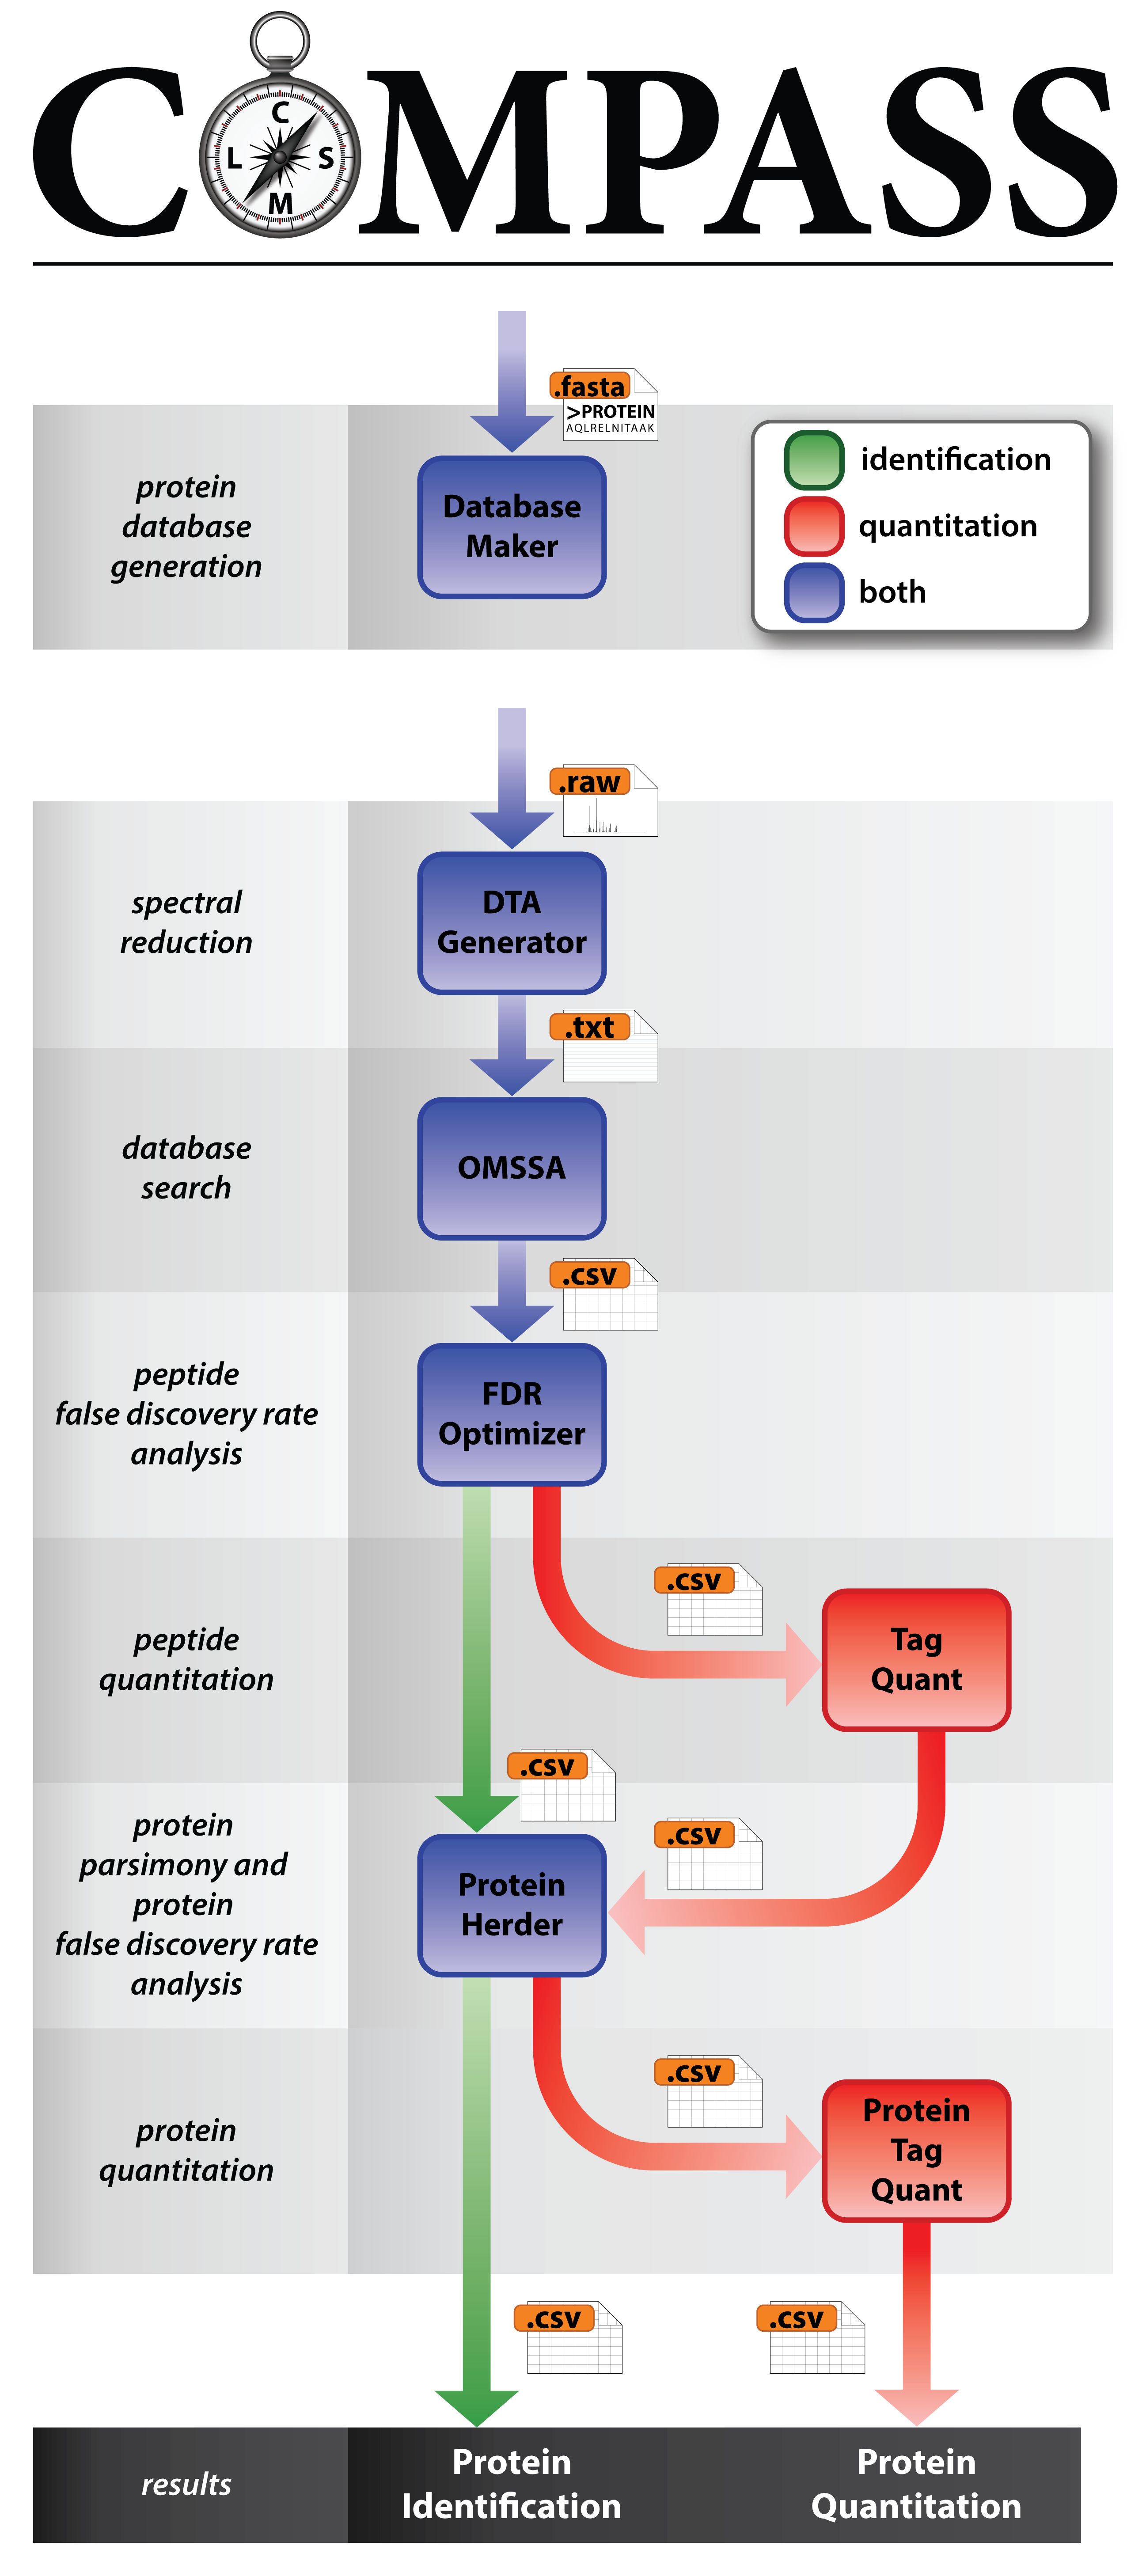
\includegraphics[width=0.5\columnwidth]{csmsl/compass.png}
	\mycaption{Analysis workflow of \compass{}}{\texttt{Database Maker} generates BLAST-formatted protein databases for \texttt{OMSSA}. \texttt{DTA Generator} converts raw instrument data to text files for searching with \texttt{OMSSA}. \texttt{FDR Optimizer} performs FDR analysis at the spectrum/peptide level, followed by protein parsimony and FDR analysis at the protein level with \texttt{Protein Herder}. For quantitation, the workflow is supplemented by \texttt{TagQuant}, which performs spectrum/peptide-level quantitation, and \texttt{Protein TagQuant}, which performs protein-level quantitation. Since publication, \texttt{Protein Herder} and \texttt{Protein TagQuant} have been combined into a new program called \texttt{Protein Hoarder}.}
	\label{fig:compass}
\end{figure}
The application contains a graphical user interface (GUI), making it very intuitive and easy to use. \compass{}  contains several other GUI programs, each corresponding to a separate step in the analysis. Users process data files through each individual program, which typically writes the result of the analysis to different files and folders on the computer. Other programs then process those result files to add additional analyses and outputs. This design enables customized analysis workflows to handle the various types of analyses commonly used (Figure \ref{fig:compass}).

\compass{} was first published in 2011, but has been substantially upgraded to improve the user experience, fix bugs, introduce new features, and speed up its execution. The program was also heavily refactored (code reorganization) to ease future maintenance. The following sections summarize the different parts of \compass{} and the improvements made to them since the initial publication.
 
\subsection*{Database Maker.}
\texttt{Database Maker} creates protein databases for target-decoy searching of MS/MS spectra. Text files containing each protein sequence, in the FASTA format, are converted to a decoy version of the same length by reversing, shuffling, or generating random amino acids.\cite{targetdecoy,targetdecoycomp,qscore} The decoy sequences are then concatenated to the input file and exported to another FASTA file. Additionally, protein sequences can be converted to the basic local alignment search tool (BLAST) format for use with OMSSA.\cite{blast} The GUI portion of the program (Figure \ref{fig:databasemaker}) has been restructured to enable multiple database files at the same time. Internally, \texttt{Database Maker} now uses the \texttt{makeblastdb} program to generate BLAST databases instead of the now depreciated \texttt{formatdb}, both of which are provided by the National Center for Biotechnology Information (NCBI).
\begin{figure}[p]
	\centering
	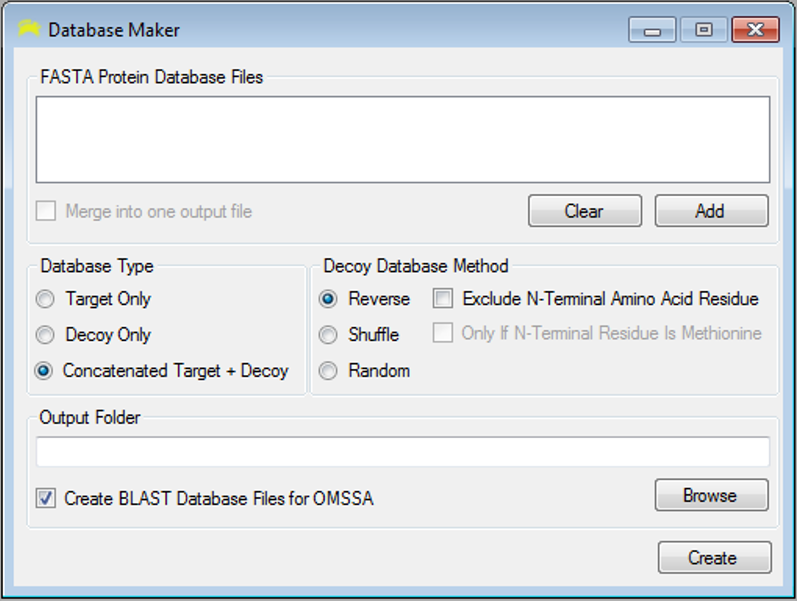
\includegraphics[width=\columnwidth]{csmsl/databasemaker.png}
	\mycaption{Database Maker}{The GUI program used to manage, construct, and modify protein databases in the FASTA format. It is capable of constructing various forms of decoy databases used for false discovery analysis. An optional BLAST database can be produced for compatibility with OMSSA searching.}
	\label{fig:databasemaker}
\end{figure}

\subsection*{DTA Generator.}
The second program in the \compass{} workflow is \texttt{DTA Generator}, which reduces LC-MS/MS spectra data to \texttt{.txt} files for database searching (Figure \ref{fig:dtagenerator}). Various peak cleaning algorithms are used to simplify spectral data prior to searching; these include removal of unreacted precursors, electron-transfer dissociation (ETD) pre-processing to remove precursors, charge-reduced precursors, and neutral losses from charge-reduced precursors.\cite{good} The outputs generated by the software are also usable by several other search algorithms. Although OMSSA is the focus, individual \texttt{.dta} files for SEQUEST or \texttt{.mgf} files for MASCOT are possible outputs.\cite{sequest,mascot}

Since the initial publication, additional spectral filters have been added to allow the user more freedom in how the spectra are processed. These include specifying neutral loss products and isobaric labels for cleaning. The most significant improvement to \texttt{DTA Generator} since publication was a dramatic decreased in execution time (\textasciitilde50X). This was accomplished by converting the code to utilize multiple processor threads, as well as algorithmic improvements to spectral cleaning. 
\begin{figure}[p]
	\centering
	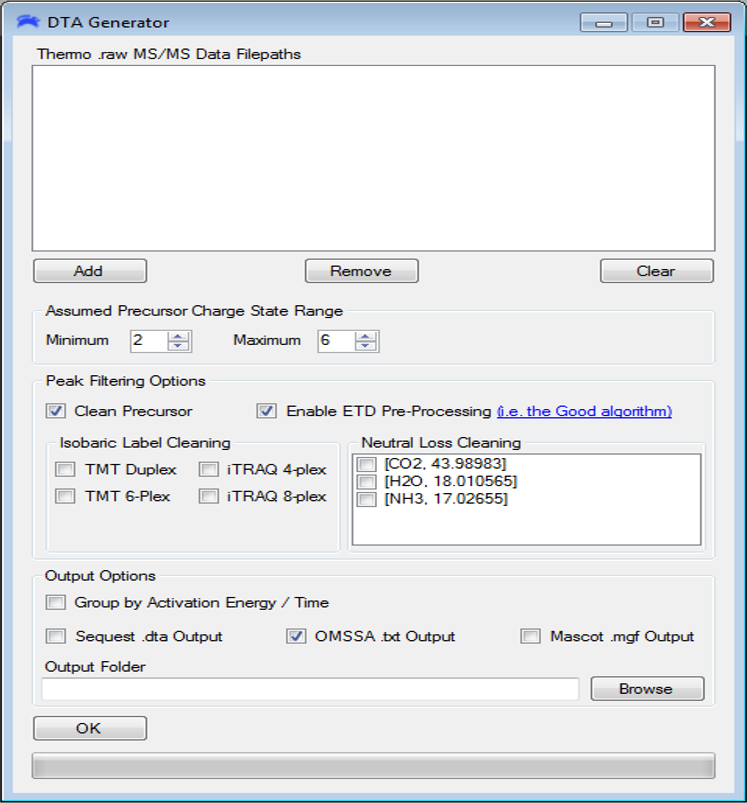
\includegraphics[width=0.8\columnwidth]{csmsl/dtagenerator.png}
	\mycaption{DTA Generator}{The program takes spectral data in Thermo's \texttt{.raw} format and generates a \texttt{.txt} of the processed spectra. Processing includes removing peaks that do not provide sequence-informative results (i.e., neutral loss). The program is capable of producing outputs for OMSSA, SEQUEST and Mascot search algorithms.}
	\label{fig:dtagenerator}
\end{figure}

\subsection*{Open Mass Spectrometry Search Algorithm.}
\texttt{OMSSA} is a database search algorithm for proteomic datasets developed at the NCBI by Lewis Geer.\cite{omssa} It uses a probabilistic scoring to associate a specific peptide sequence to an experimental spectrum. The program assigns an expectation value (e-value) to each peptide spectrum match (PSM) generated, stating the probability of matching that sequence to the spectrum by random chance. The smaller the e-value, the higher the confidence that peptide sequence produced the MS/MS spectrum. Further statistical analysis is performed in the \texttt{FDR Optimizer} program, discussed below. OMSSA provides the option to produce a \texttt{.csv} output of all the PSMs generated. This format is the basis for all the other programs in \compass{}. It is easily opened and manipulated by spreadsheet programs (e.g., Microsoft Excel) and is human readable. This is in contrast to a majority of other proteomic software, where \texttt{.xml} or a proprietary format are used. Those formats make modifying and parsing the data more difficult than a \texttt{.csv} file.

\subsection*{High Throughput Condor for OMSSA.}
Arguably the biggest improvement to \compass{} since publication is the addition of the High Throughput Condor (HTCondor) system for improving OMSSA searching times. In brief, HTCondor is a computational management system for scheduling processing jobs across a distributed network of computers. Computers voluntary join a HTCondor network which enables them to donate their free CPU cycles to other processes, increasing the overall processing power of the network. This is ideal for large universities, where there is a large number of computers on a common network, and a majority of those computers (e.g., computer labs, servers, kiosks, office computers) are not in use twenty-four-seven. The HTCondor system intelligently monitors CPU activity on each attached computer, and given a certain amount of inactivity, reassigns its CPU to process jobs waiting in a global queue. If HTCondor detects new local activity on that computer (e.g., keyboard or mouse movement, a local processing job, etc.), it will either pause the global job, or automatically transfers it to another inactive computer. Given the large size of the HTCondor network on the University of Wisconsin-Madison campus (\textasciitilde7,000 CPUs) there is a high probability that there will always be multiple computers available for analysis. This large network provides million of CPU hours to researches all across campus. From the HTCondor website, they state that ''from July 2011 to June 2012, the [Center for High Throughput Computing] provided 70 Million CPU hours to campus researchers and off-campus collaborators.''

Shortly after \compass{} was published, I developed a GUI program called \texttt{Coondornator} to provide a method for searching MS/MS data \emph{via} OMSSA over the University of Wisconsin-Madison's HTCondor network. The program first transfers \texttt{.dta} files (generated by \texttt{DTA Generator}) from a user's computer to the Coon Group computer cluster, which is its own 17-CPU HTCondor network. If these computers are idle, they automatically start processing each submitted OMSSA job. If more than 17 OMSSA searches are submitted at once, overflow jobs are automatically routed to the Center of High Throughput Computer (CHTC) HTCondor cluster (\textasciitilde6,800 CPUS) for analysis. It is common to have 50-100 OMSSA searches going at any give time. When the OMSSA searches are completed, the resulting \texttt{.csv} file containing all the PSMs are transferred back to the Coon Group computer cluster for storage. This program provides a seamless integration between the HTCondor network and an end user's computer, making high throughput computing no harder than running a program on their computer. The Coon Group routinely searches thousands of \texttt{.dta} files containing million of spectra on the HTCondor network each week.

Previously, users would search all the MS/MS spectra from a single LC-MS/MS experiment on their desktop computers. Now with \texttt{Coondornator} and HTCondor, a single LC-MS/MS experiment is broken up into smaller sets of spectra (e.g., 1000 spectra per set), searched individually, and then recombined when all the searches are complete. This represents a significant throughput gain compared to searching files on individual desktop computers. With execution times decreasing on average about 30-50X. For example, it would take about 30-40 minutes on a desktop computer to search all the MS/MS spectra from a one hour LC-MS/MS experiment of a tryptic digestion of whole-cell yeast cells. In contrast, if all the MS/MS spectra were split into groups of 1000 spectra each, and searched using \texttt{Coondornator} over the distributed HTCondor network, the same results could be generated in \textasciitilde1 minute, a 30X decrease in execution time.

\subsection*{FDR Optimizer.}
\texttt{FDR Optimizer} filters PSMs generated from \texttt{OMSSA} to control for false identifications (Figure \ref{fig:fdr}). The program maximizes the number of true positive identifications at a given false discovery rate (FDR), typically set to under 1\%. \texttt{FDR Optimizer} can work on either low-resolution MS data with a simple e-value filter, or on high-resolution MS data with a two dimensional filter on precursor mass error and e-value. To use \texttt{FDR Optimizer}, both target and decoy protein sequences have to be searched with \texttt{OMSSA} on the same set of spectra for adequate false discovery filtering. 
\begin{figure}[p]
	\centering
	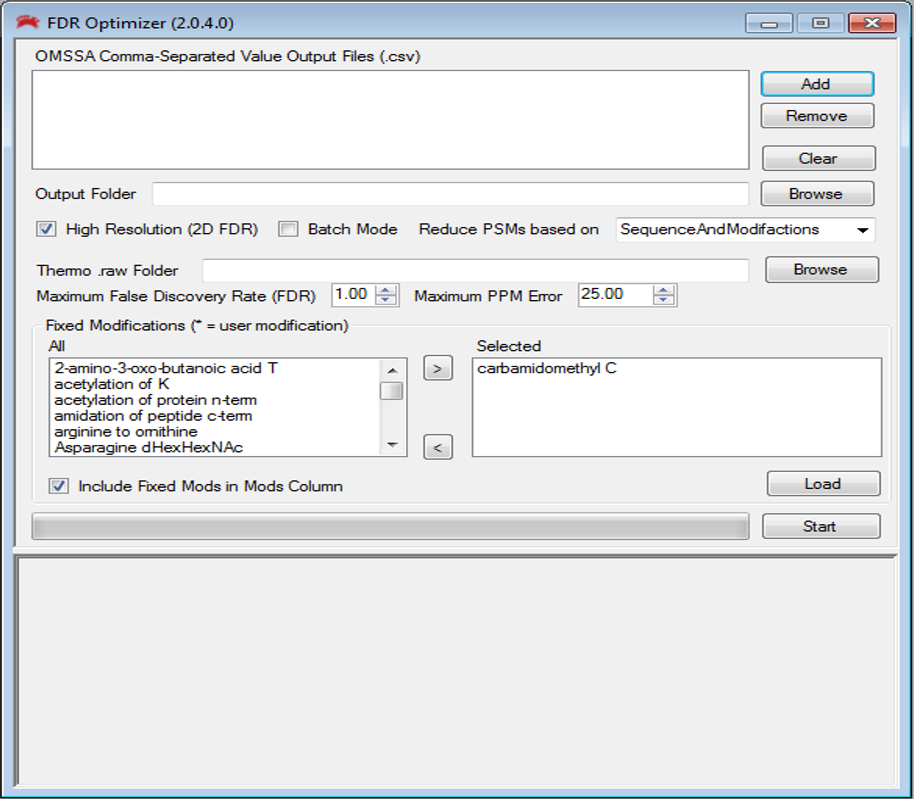
\includegraphics[width=\columnwidth]{csmsl/fdr.png}
	\mycaption{FDR Optimizer}{The new GUI for \texttt{FDR Optimizer}, this version combines all four versions into one program for a simplified user experience.}
	\label{fig:fdr}
\end{figure}

For low-resolution datasets, PSMs are first loaded into the program and the best scoring PSM (i.e., lowest e-value) for each spectrum is saved and all other PSMs are discarded. The remaining PSMs are then sorted on their e-value, from smallest to largest. Each PSM also has a flag to indicate whether it resulted from a target protein or a decoy protein. A counter for both the number of targets ($T$) and decoy ($D$) peptides identified is kept as the program iterates over the sorted PSMs. When the false discovery rate (Equation \ref{eq:fdr}) increases over some specified value (e.g., 1\%), the program stops the iteration.
\begin{equation}
FDR =\frac{D}{T + D}
\label{eq:fdr}
\end{equation}
The PSMs that represent the true identifications and which have already been processed are then outputted to a \texttt{.csv} file. Known decoy peptides that pass this filter are exported to a decoy-specific \texttt{.csv} file that is used later for protein-level FDR analysis.

High-resolution MS datasets can be processed with an additional filter to increase the number of identifications. First each PSM is read into the program and its precursor mass error is determined from the MS spectrum that triggered the MS/MS event. The median precursor mass error of all PSMs is then computed and each PSM is corrected by this value. This process corrects any systematic mass error the mass spectrometer had, and usually reduces the mass errors to <5 ppm. \texttt{FDR Optimizer} then iteratively sets a maximal ppm error allowed (i.e., from 1 to 100 ppm), and filters the PSMs to contain only precursor mass errors lower than the maximum. These filtered PSMs are then processed identically to the low-resolution analysis described above. This whole process is then repeated with a slightly larger maximal ppm error, and the number of identifications is recorded. The program tries all possible maximal ppm errors and reports the ppm error that produced the most true identifications at the end. This maximizing algorithm increases the number of true identifications produced over the simple low-resolution filter by roughly 10-15\%.

Since publication, \texttt{FDR Optimizer} has been completely rewritten. Previously, four separate programs were used and maintained: \texttt{Low-Resolution FDR Optimizer}, \texttt{FDR Optimizer}, \texttt{Batch Low-Resolution FDR Optimizer}, and \texttt{Batch FDR Optimizer}. The current version simplifies the user experience by combining all four programs into one, with simple option check-boxes to indicate the desired analysis (Figure \ref{fig:fdr}). Improvements to the FDR analysis and maximizing algorithms have also lead to large decreases in execution times (\textasciitilde10-20X).

\subsection*{TagQuant.}
The \texttt{TaqQuant} program extracts and processes isobaric labeling quantitative information from MS/MS spectra (Figure \ref{fig:tagquant}). It is compatible with both common types of isobaric labels, TMT and iTRAQ.\cite{tmt,itraq} \texttt{TagQuant} obtains intensities of the reporter ions of interest from the raw data. These intensity values are subsequently denormalized by multiplying by the ion injection time to yield the number of ion counts detected, a quantity which can be fairly compared across different spectra and analyses. Purity correction is then applied using user-specified purity data provided by the manufacturer.\cite{itracker} Finally, normalization is performed such that the total intensity of each tag is equal, accounting for differences that arise when samples are mixed.
\begin{figure}[p]
	\centering
	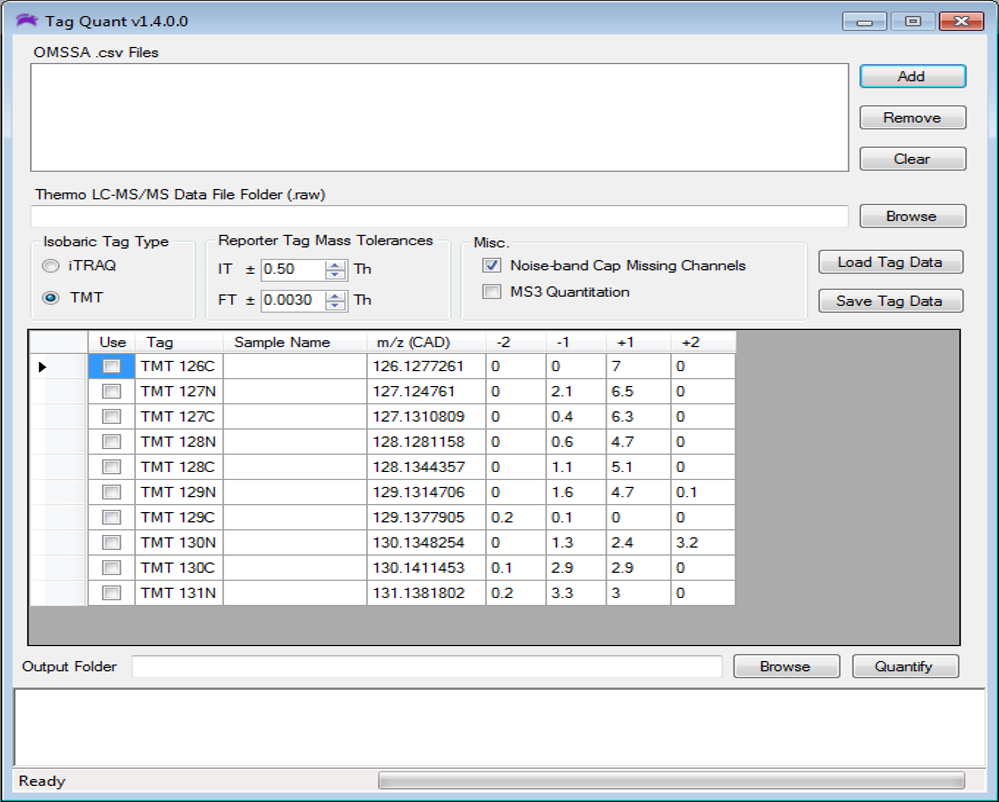
\includegraphics[width=\columnwidth]{csmsl/tagquant.png}
	\mycaption{TagQuant}{The updated GUI for \texttt{TagQuant} allows users to specify the exact labels used and their relative purities. Options for noise-band capping missing channel and quantifying from an MS$^3$ scan are also included.}
	\label{fig:tagquant}
\end{figure}

Numerous improvements have been made to the publication version of \texttt{TaqQuant}. With the advent of high-resolution TMT tags, where two quantiation channels are separated by a very small mass difference (6.32 mDa), additional logic had to be added to handle it.\cite{tmt8,tmt82} Users also started to mix and match channels between different manufacturing lots, resulting in non-standard purity values. This, and other issues, were corrected by providing the user full control over which labels they used to quantify and their respective purities. This change also enables \texttt{TagQuant} to handle any type of isobaric label later developed without making changes to the program itself.

Another heavily used feature that was added was capping missing channels with the noise-band intensity. Sometimes a peak at an expected isobaric tag \mz{} is not present in the MS/MS spectra. Before, this missing value was set to $0$, which would drastically distort the ratio between quantitation channels. In the updated version, \texttt{TagQuant} assigns the missing value to the noise level at the \mz{}. This conservative approach mitigates the distortion of ratios between quantitative channels. An additional feature that was added was enabling quantitation from MS$^3$ spectra. This is the result of purification methods for improving the interference problem of isobaric labels, such as QuantMode and the MS$^3$ methods.\cite{quantmode,ms3}

\subsection*{Protein Hoarder.}
\texttt{Protein Hoarder} infers the most likely proteins identified based on the peptides validated by \texttt{FDR Optimizer} (Figure \ref{fig:hoarder}). The program was initially called \texttt{Protein Herder}, but the program was completely rewritten after publication, and the name was changed to indicate that it is a new program.
\begin{figure}[p]
	\centering
	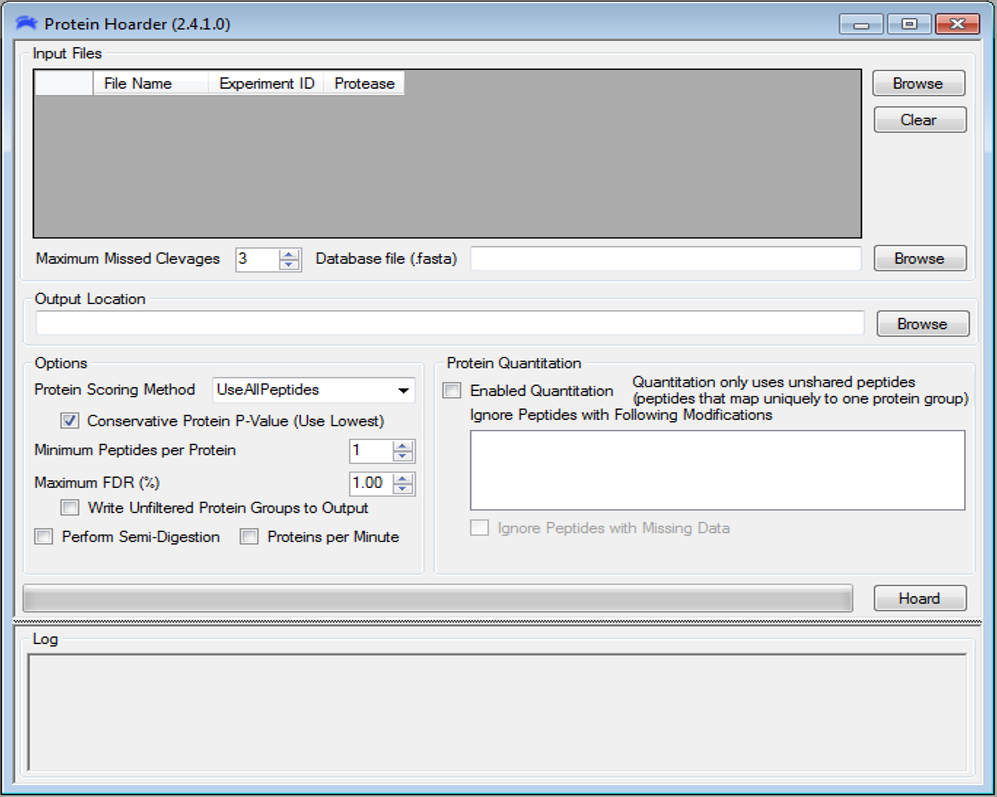
\includegraphics[width=\columnwidth]{csmsl/proteinhoarder.png}
	\mycaption{Protein Hoarder}{The new version of \texttt{Protein Herder} which assembles peptide identifications into protein groups. This version also performs protein quantitation at the same time the protien groups are being assembled.}
	\label{fig:hoarder}
\end{figure}
In this program, peptides are assembled into protein groups based on the law of parsimony, i.e., minimizing the number of protein groups while accounting for all the identified peptides. False discovery analysis is also performed at the protein-level, along with quantitative analysis if requested. The outputs of the program include a \texttt{.csv} file containing all the identified protein groups, along with which peptides are mapped to the groups.

The biggest change between the original and current version is how the peptides are found within the candidate proteins. Previously, each peptide sequence was searched against the whole protein database using brute force. For large databases such as the human proteome, the number of proteins could reach over 150,000 when isoforms and both target and decoy proteins are considered. Even if only 20,000 PSMs were identified, that means 30 billion string comparisons must be made (20,000 x 150,000). This made the original program very slow, and could take up to half a day to assemble protein groups for a human sample. The new algorithm forgoes the string search and uses enzymatic cleavage of the proteins to find the associated peptides. The program preforms an \emph{in silico} digestion of all the proteins and if a generated peptide matches one of the input PSMs, that protein is saved. This process greatly speeds up the whole program, and the same human sample that took half a day to assemble now takes less than 2 minutes. 

Assembled protein groups are further filtered for false discovery using a similar method to \texttt{FDR Optimizer}. Here, the p-value of the protein group (which is the product of all the peptide's e-values) is the ordering metric and the groups are filtered to a specified FDR (e.g., 1\%). In the publication version of \compass{}, there was another program that handled protein quantitation (\texttt{Protein TagQuant}) by summing up all the peptide quantitation for a individual protein group. Peptides that are not shared between protein groups (i.e., a unique peptide to the protein group) have their quantitation summed and reported for the protein group. This program was embedded into \texttt{Protein Hoarder} since all the required information for quantitation was already present in the program. This removed the need for using \texttt{Protein TagQuant} altogether, and it was removed from \compass{}. 

\subsection*{LoToR.}
The final program in \compass{} was not present in the initial version. This program is called \texttt{LoToR} (\underline{Lo}calize \underline{To} \underline{R}esidue) and improves the localization of post translational modifications to specific residues on peptides and proteins. Although \texttt{OMSSA}, and other search algorithms, are capable of identifying modification events on peptides, it often does not place the PTM on the correct residue. To address this, \texttt{LoToR} was created to add more rigorous statistical power in localizing PTMs to specific sites. 

\texttt{LoToR} is uses the AScore algorithm as the primarily metric for assigning statistical confidence.\cite{ascore} In brief, for each PSM that contains a PTM, all possible peptide isoforms are generated. Each of these isoforms represents the unique combination of PTMs applied to every possible site on the peptide. Then each isoform is fragmented \emph{in silico} and matched to the MS/MS spectrum. After matching, each isoform is compared to every other isoform generated, and the set of fragments that can distinguish them apart are called 'site-determining fragments' (SDFs). The number of identified SDFs for each isoform is then compared, and the two isoforms that have the biggest difference in the number of identified SDFs is declared the best possible isoform. The AScore for this pair of isoforms is then computed, and if the value is above some defined value (typically 13), it is declared localized. \texttt{LoToR} is capable of handling any modification (e.g., phosphorylation, acetylation, ubiquitination, etc.). 

\section{CSMSL: C\# Mass Spectrometry Library}
Mass spectrometry-based proteomics is a relatively young field that is rapidly evolving and new techniques and technologies are consistently being developed, prompting the need for custom software tools to analyze the data. There are typically three ways to analyze a proteomic dataset: 1) process it through a full-fledged GUI program that has already been developed, 2) manually process the data, or 3) extract data with software tools and analyze with other software (e.g., Microsoft Excel). Often a mixture of these three processes are needed to fully analyze a dataset. However, sometimes a complete GUI program is not available for a specific type of data analysis, or, due to the complexity of the data, manual analysis of a dataset in Excel or through a spectrum browser (e.g., Thermo XCalibur) is a daunting and time-consuming task. These situations are ideal for a custom analysis program that could facilitate the analysis. Unfortunately, creating custom programs is not straightforward: 1) not every researcher knows how to program, and 2) there isn't a free, simple programming environment for accessing and manipulating such complex data. The first problem is not easily addressed, but the second one is. Although there are many tools available for MS analysis on the internet, most are difficult for novice programmers and are challenging to adapt to a specific need. To fill the gap, I have designed a large proteomic programming library to simplify the data management and manipulation of large-scale proteomic data. It is written for Windows using the .NET Framework V4.0 in the C\# programming language. It is called C\# Mass Spectrometry Library (\csmsl{}) and is freely available at \url{https://github.com/dbaileychess/CSMSL}.

The goals of \csmsl{} are to provide an easy-to-use, powerful, feature-rich library of .NET C\# objects and methods to enable even novice programmers the ability to analyze proteomic data quickly. Simplicity is key. Calculating the mass of the peptide sequence 'CSMSL' only requires the following two lines:
\lstset{style=sharpc,numbers=left,numberstyle=\small,keywordstyle=\color{blue},
morekeywords={Peptide,Protein,Console,Protease,ChemicalFormula,List,FastaReader,MSDataFile,MSDataScan}}
\begin{lstlisting}
Peptide peptideA = new Peptide("CSMSL");
Console.WriteLine(peptideA.MonoisotopicMass);
// outputs : 539.20835516707
\end{lstlisting}
In addition to simple syntax, \csmsl{} is designed with performance in mind, allowing even computationally intensive calculations to be completed quickly. For example, a complete yeast database (6,627 proteins) can be loaded from a FASTA file, digested with trypsin (up to 3 missed cleavages, 5 to 35 amino acids in length) in under 2 seconds. If the calculation for the [M+H]$^+$ \mz{} of each of the 913,740 resulting peptides is included, the total time only goes up to 4 seconds (this includes full chemical formula determination). While \csmsl{} is not expected to meet the performance of advanced compiled languages (e.g., C/C++, Fortran, etc.), its adequate performance plus simplicity of use are sure to be helpful in analyzing data in new and creative ways without significant overhead.

The following sections will succinctly 1) describe the design of the library, 2) show a few example code segments indicating its use, and 3) highlight various features and abilities of the library.

\subsection*{CSMSL Design.}
The \csmsl{} package is divided into three projects. The main project is the library itself (\texttt{CSMSL.csproj}) which contains all the code and objects to program with. This project will be described in greater detail in the sections to follow. The other two projects are primarily used for teaching and development purposes, and will be described here. 

The teaching project is \texttt{CSMSL.Examples.csproj}, which contains short segments of code to show the intended use of the library. It is written to aid novice programmers in learning how to program better and how to use the library. It covers a series of example code to demonstrate how to create peptides and proteins, digest proteins, fragment peptides, read in spectral data, among many others. This project is completely separate from \csmsl{} and is only used to demonstrate the features of the main library. 

The development project is \texttt{CSMSL.Tests.csproj}, which hosts all the unit tests for the library. A unit test is a short piece of code that tests one, and only one aspect of the library, hence the term 'unit'. In brief, a short segment of code is written to preform some action (e.g., digest a protein), and the final line contains an assertion statement, declaring that some value needs to possess some trait (e.g., that 5 peptides are produced from a digestion of a certain protein). These assertions can be as simple as an equality ($numOfPeptides == 5$), a comparative condition ($numOfPeptides < 5$), or much more advanced comparisons. Regardless, the point of unit tests is to provide fine grain support and testing for the main project. If any source code is added to the project or a portion of code is changed, all the unit tests report back to the developer if their one piece of functionality is still producing the same result. If not, the developer has a good idea of where the new bug is introduced as only certain unit tests will fail. This helps ensures that new features do not affect other parts of the library or produce unintended bugs. \csmsl{} is heavily tested, especially on the components that are most commonly used.

There also exists a handful of other projects that supply support for third-party tools and access to raw spectral data from different MS vendors. These are located under the \texttt{CSMSL/IO} directory and can be added to a project when needed. The projects that support reading in raw spectral data will be discussed in the features section below. Since \csmsl{} has been developed, it has been heavily incorporated into the source code of \compass{}. This helps simplify every program within \compass{}, as many redundant sections of code were replaced by objects from \csmsl{}. It also helps speed up bug fixes and feature additions, as all programs that use \csmsl{} will benefit from improvements in its code.

\subsection*{CSMSL Examples.}
Functional coding examples are a great way to dive into any programming language/library. \csmsl{} provides a number of example programs, contained within the \texttt{CSMSL.Examples} project, so that people can learn the tools and experiment with different features. Below are a series of examples showing the simplicity and power \csmsl{} offers. All of the examples are written in the C\# language and should be straightforward enough that even non-programmers should be able to follow them.

We will start with the most basic, but most commonly used features: proteins and peptides. The following code first constructs a new peptide object in memory, labels it as '\texttt{peptideA}' and then prints its monoisotopic mass to the console window.
\begin{lstlisting}
Peptide peptideA = new Peptide("FLTTSNALKEN");
Console.Write(peptideA.MonoisotopicMass);
// outputs: 1236.635016661
\end{lstlisting}
Of course there are a plethora of tools and websites that could calculate the monoisotopic mass of a peptide sequence, but the novel aspect is its simplicity and the ability to programmatically control it.

Peptides and proteins can be modified post transitionally and \csmsl{} enables easy methods for modifying peptides. Taking the previous example further, to modified the serine residue ('S') with a phosphorylation is easy:
\begin{lstlisting}
Peptide peptideA = new Peptide("FLTTSNALKEN");
ChemicalFormula phospho = new ChemicalFormula("HPO3");
peptideA.SetModification(phospho, 'S');
Console.Write(peptideA.MonoisotopicMass);
// outputs: 1316.60134718175
\end{lstlisting}
Only two new lines are inserted. Line 2 creates the phosphorylation modification (labeled as '\texttt{phospho}'), and introduces another \csmsl{} object called \texttt{ChemicalFormula}, which represents a chemical structure. The third line sets the '\texttt{phospho}' chemical formula to modified all the serine residues in \texttt{peptideA}. Since there is only one serine in \texttt{peptideA}, only one phosphorylation is added, resulting in a mass of $1316.601347$.

Another important feature often used is protein digestion. In nature, peptides often arise from the proteolyic digestion of intact proteins by proteases, such as trypsin. \csmsl{} can do the same thing \emph{in silico} that is done in a test tube. Below is an example of a tryptic digestion of a single protein. It produces a list of \texttt{Peptide} objects which are then printed to the screen.
\begin{lstlisting}
Protein proteinA = new Protein("MMGFKQLITTGSSSRSSSSKDTSST");
List<Peptide> peptides = proteinA.Digest(Protease.Trypsin);
Console.Write(peptides);
// outputs: MMGFK, QLITTGSSS, SSSSK, etc...
\end{lstlisting}
The first line creates a new \texttt{protein} object in memory, just like the peptide example above. The second line takes the created protein (\texttt{proteinA}) and performs a digestion with trypsin. The result (the left hand side of the equation) is a list of \texttt{Peptide} objects. The final line then takes all those peptide sequences and prints them to the screen. This is a simple digestion, but there exist many more options, such as maximum and minimum peptide length, max missed cleavages, partial digestion, etc. All these options will not be explored here, but almost anything you could do on a physical protein/peptide, can be performed \emph{in silico} using \csmsl{}.

\subsection*{Full Proteome Tryptic Digestion Example.} The code section shows a complete example of a tryptic digestion of a yeast proteome. Its inclusion here is to demonstrate that a fairly complicated task can be performed with only a few lines of code that should be easily understandable to a novice programmer.
\begin{lstlisting}
using (FastaReader reader = new FastaReader("yeast.fasta"))
{
 Protease trypsin = Proteases.Trypsin;
 int max = 3;  // Maximum number of missed cleavages
 foreach (Protein protein in reader.ReadNextProtein())
 {
  foreach (Peptide peptide in protein.Digest(trypsin, max))
  {
    Console.WriteLine(peptide.MonoisotopicMass);  
  }
 }
}       
\end{lstlisting}
Line 1 opens up a connection to a protein database file named ''yeast.fasta'' located on the computer. The \texttt{FastaReader} object provides methods for reading and accessing proteins contained in a FASTA-formatted file. The third line sets up a variable that represents the typsin protease. Line 4 sets another variable defining the maximum number of missed cleavages allowed for the digestion. The fifth line iterates over each \texttt{Protein} within the FASTA file, by calling the \texttt{ReadNextProtein()} method. The lines 6 through 11 are then performed for each protein read in by line 5. Line 7 iterates over every peptide generated from the digestion of the protein by trypsin and a maximum missed cleavage of three. Again, lines 8 through 10 are repeated for every generated peptide. The last important line is line 9, where the peptide's monoisotopic mass is written to the console window on the computer. In only 12 lines of code, a complicated task is accomplished using \csmsl{} objects and methods. Similarly, other proteomic analysis and computations can be expediently coded and performed. These examples can be found in more details in the \texttt{CSMSL.Examples.csproj} project file.

\subsection*{CSMSL Features and Objects.}
The \csmsl{} library has too many features to list in full, so only a few of the most important features will be highlighted here. Since this is primarily a proteomic library, it will start off with proteins and chemicals and then transition to spectral classes. 

Starting from the smallest object and growing bigger, elemental isotopes represent the basic building block of everything else that has mass. Each isotope has a few intrinsic properties, most importantly its mass and the element it belongs to. A single element may contain a set of different isotopes (e.g., $^{12}C$, $^{13}C$, and $^{14}C$), and the naturally most-abundant isotope is declared the principal isotope of the element. Thus elements and their most abundant isotopes are interchangeable with each other (i.e., $^{12}C$ and $C$ refer to the same object). When other isotopes are needed, you need to specify which isotope you want to use (e.g., $C\{13\}$ mean you want $^{13}C$ instead of $^{12}C$). This feature is important because stable isotope quantitative labeling is a very common analysis, and I wanted to design the library with it in mind. All the elements, and thus isotopes, are assembled into the periodic table of elements for easy access.

In \csmsl{}, chemical formulas are represented as a set of isotopes without any spatial connectivity. Keeping the three dimensional structure of molecules is not an important aspect of most proteomic work, and I purposefully left this out in favor of speed and memory savings. Additionally, a chemical formula generator is available to list all possible chemical formulas when given an exact mass. Such features are used to indentify unknown peaks in high-resolution mass spectra. The mass of a chemical formula is the simple summation of all of its isotopes. Almost every other object in this library is a chemical formula (e.g., proteins, peptides, amino acids, modifications, etc.)  with additional properties of its own. Amino acids are simply a chemical formula with a character symbol to represent which one it is. The 20 common amino acids are prebuilt by the library and ready to use, but custom amino acids can be added easily.

Probably the most important classes in the library are the protein and peptide classes. Since both a protein and peptide can be thought of as a string of amino acids, both classes are modeled off a single base class called \texttt{AminoAcidPolymer}. This class can be thought of as an fancy array of amino acids, spanning from the N-terminus to the C-terminus. Each location on this array (i.e., amino acids or termini) can be modified by a chemical formula. The mass of the \texttt{AminoAcidPolymer} is again the summation of all its amino acids and modifications. Peptides have special methods for producing fragments ions (e.g., a, b, c, x, y, z-type, as well as others). Fragment ions are also chemical formulas, but they keep track of what amino acids and modifications are contain in each fragment. This is particularly useful when matching fragment ions against a mass spectrum, as it fully annotates the spectrum during the matching steps. Proteins have methods for proteolytic digestion by any enzyme. Users can also define their own proteases to use, and they will be compatible with all the features of digestion (e.g., missed cleavages, min/max lengths, semi-digestions, etc.).

Finally, a set of spectral-related classes are included to provide easy access to spectral data. In \csmsl{} spectra are comprised of a ordered list of \texttt{Peaks}, which represents the \mz{} and intensity of the peak. These \texttt{Peaks} objects can be extended to contain additional information (e.g., charge, noise, baseline intensity, etc.) provided by the instrument. The \texttt{Spectrum} class contains the data of a specific spectrum and provides a series of methods for easy data access. Since a large part of proteomic analysis is looking for peaks within a spectrum, probably the most important method is the \texttt{GetClosestPeak()} method. This uses a binary-search algorithm to quickly find the closest peak to a given \mz{} value, and this operation takes on average $O(\log N)$ time, where $N$ is the number of peaks in the spectrum. Even with complex spectrum of 1,000 peaks, it only takes about 7 comparisons to locate a peak.

\subsection*{Spectral Data Access.}
A very useful feature \csmsl{} provides is access to raw spectral data collected by the MS. Instrument vendors usually offer an application programming interface (API) for accessing data from their propriety data formats (e.g., \texttt{.raw} for Thermo, \texttt{.d} for Agilent, etc.). While it is possible to use them on own, a few factors make them difficult to implement. First, they are geared to more advanced programmers and often have incomplete documentation. This makes learning how to access the data difficult, even for good programmers. For people who don't know how to program at all, it would be very difficult to understand and make work. Secondly, each instrument vendor creates their own API which is incompatible with everyone else's. Thus if you desire to analyze two different types of data with your program, you'll have to use both APIs to achieve the same result. This additional code can often lead to bugs and frustration. Lastly, you have to be an expert in each API in order to fully use their capabilities. \csmsl{} solves these issues by having a single and simple interface for accessing the data, no matter where or how the data was produced.

The following example shows how to read in every MS spectra from a \texttt{.raw} file generated from a Thermo mass spectrometer.
\begin{lstlisting}
MSDataFile dataFile = new ThermoRawFile("somerawfile.raw")
dataFile.Open();                   
foreach (MSDataScan scan in dataFile)
{             
    Console.WriteLine('Number of Peaks: '+scan.PeakCount);
}
\\ outputs:
\\   Number of Peaks: 1052
\\   Number of Peaks: 523
\\   etc..
\end{lstlisting}
First, in line 1 a mass spectrum data file is constructed from a file on the computer, named ''somerawfile.raw''. The second line opens a connection to the file, and the third line iterates over each MS scan within that file. The number of peaks contained within that scan is then printed to the screen. The beauty of this example is that the first line could be changed to:
\begin{lstlisting}
//MSDataFile dataFile = new ThermoRawFile("somerawfile.raw")
MSDataFile dataFile = new AgilentDDirectory("somerawfile.d")
\end{lstlisting}
and the program would continue to work, even though it is now accessing MS data collected by an Agilent mass spectrometer. Having this sort of flexibility built in from the start enables programmers to program their tools once and have it work with data from any source supported. As of this publication, only Thermo \texttt{.raw}, Agilent \texttt{.d} and \texttt{.mzML} formats are supported. However, other vendors could be added in the future without breaking code. While there are too many features to be fully explained here, the concept of a simple and consistent way to access spectral data is a key component of \csmsl{}. 

\bibliographystyle{ieeetr}
\bibliography{csmsl}